\chapter{O ciclo de vida do produto na I4.0}
\label{cha:ciclo-de-vida}
	
	Este capítulo visa trazer discussões sobre o impacto do amplo compartilhamento da memória digital do produto ao longo da cadeia de suprimentos por meio de serviços na Indústria 4.0.
	
	São abordadas possíveis mudanças na curva de ciclo de vida do produto e o surgimento de novos modelos de negócio baseado em dados (\textit{data-driven}).
	
	Uma visão da MDP sobre o eixo ``Ciclo de Vida e Cadeia de Valor'' do RAMI4.0 é abordada, discutindo melhor o porquê e as atribuições dos AASs como ``tipos'' e como ``instâncias''.

\section{Ciclo de vida do produto no RAMI4.0}
	
	O modelo do RAMI4.0 apresenta um eixo de ciclo de vida generalizado, derivado da norma IEC 62890 \cite{adolphs2015rami}. O objetivo deste eixo é representar o ciclo de vida de um Componente I4.0 ao longo de toda a sua cadeia de valor.
	
	Os ``tipos'' estão presentes desde a concepção/conceitualização até os primeiros protótipos/testes. O ``tipo'' de um ativo é definido pelas suas propriedades e funcionalidades distintas. Todos os itens que são criados ao longo do projeto de um produto (e.g., desenhos em CAD, manuais, \textit{softwares}, etc) são incorporados ao ``tipo'' do ativo. Informações externas associadas ao ativo que são criadas ao longo de seu desenvolvimento como informações de \textit{marketing} também são incorporadas ao ``tipo''.
	
	As instâncias são criadas, produzidas ou fabricadas com base nas informações de um ``tipo'' de ativo. Informações específicas sobre produção, logística, qualidade e testes são associadas à ``instância'' de um ativo. Nesta fase, os dados de uso são coletados e associados para então poderem ser armazenados na MDP de cada ativo e serem compartilhados com outros parceiros ao longo da cadeia de suprimentos. 
	
	O histórico completo do ciclo de vida do produto está associados à combinação entre ``tipo'' e a ``instância'' de um determinado produto. Estes dados podem ser aproveitados de forma inteligente para a geração de valor, gerando assim novos modelos de negócio.
	
	Os relacionamentos entre ``tipos'' e ``instâncias'' são cíclicos e possibilitam a retroalimentação de informações. Para os ativos de um produto, por exemplo, informações sobre seu uso e sobre manutenções realizadas podem ser armazenadas na MDP e assim auxiliar em melhorias no seu próprio processo de fabricação, além de ser fonte de dados para o desenvolvimento de novas versões aperfeiçoadas do mesmo produto, gerando um novo ``tipo''.
	
	Portanto, esse fluxo de informações entre ambas as fases de um produto são essenciais para a melhoria de seu próprio projeto. A \autoref{fig:aas-lifecycle} ilustra como ocorre a instanciação (criação de uma instância a partir de um tipo) e o uso da MDP das ``instâncias'' para a criação de novas versões de um ``tipo''.
	
	\begin{figure}[htb!]
		\centering
		\label{fig:aas-lifecycle}
		\includegraphics[width=1\textwidth]{aas-lifecycle}
		\caption{Ciclo de vida do produto.}
	\end{figure}

\section{Transformação da competitividade por meio produtos inteligentes}

	O extenso uso de sensores e recursos de conexão permitem com que produtos se tornem ``inteligentes'', isto é, ganham a capacidade de se comunicar com outros dispositivos e compartilhar informações de estado.
	
	A ascensão de produtos inteligentes no contexto da Indústria 4.0 trazem duas formas básicas de agregação de valor ao produto por meio do compartilhamento da MDP: as \textbf{melhorias de projeto} e as \textbf{melhorias operacionais}.
	
	Estes novos tipos de produtos e a possibilidade de exploração de seus dados alteram a estrutura da indústria e a natureza da concorrência, expondo as empresas a novas oportunidades e ameaças competitivas \cite{porter2014smartproducts}.
	
	Estes produtos passam a combinar hardware, sensores, armazenamento de dados, microprocessadores, software e conectividade de inúmeras maneiras. Esses “produtos inteligentes e conectados” possibilitados por grandes melhorias no poder de processamento e miniaturização de dispositivos e pelos benefícios de rede da conectividade sem fio onipresente estão desencadeando uma nova era de competição.
	
\section{Uso da MDP na melhoria de projeto do produto}

	A extração de informações da MDP auxilia no desenvolvimento de novas versões com ``tipos'' aprimoradas. Novos ``tipos'' aprimorados significam a melhoria de projeto do produto.

	Com os ciclos de vida do produto cada vez mais curtos e cadeias de suprimentos cada vez mais complexas, explorar o registro de informações do produto pode garantir uma posição competitiva de uma empresa comercial frente aos competidores.
	
	Além disso, a memória digital do produto abre novas possibilidades em relação ao combate à pirataria e falsificação de produtos, na proteção ao consumidor e na garantia de qualidade do produto \cite{wahlster2007digitalmemory}.
	
	\citeonline{porter2014smartproducts} e \citeonline{porter2015smartproducts} classificam as funções e capacidades dos produtos em quatro áreas: monitoramento, controle, otimização e autonomia. Por meio da análise da descrição das funcionalidade e capacidades de cada área, foi feito um mapeamento dessas funcionalidades para o contexto do eixo ciclo de vida e cadeia de valor do RAMI4.0.
	
	As funcionalidades e capacidades dos produtos no que diz respeito à melhoria de projeto foram então classificadas de acordo com as seguintes categorias:
	
	\begin{itemize}
		\item Identificação e reparo de falhas de projeto;
		\item Adição/remoção de funcionalidades;
		\item Melhorias de experiência do usuário com o produto;
		\item Geração de indicadores.
	\end{itemize}

	Estas categorias permitem segregar os dados de acordo com seus respectivos objetivos ao serem inseridos no projeto de um produto. Além disso, as categoriais dão indícios de possíveis informações genéricas a serem armazenadas pelo produto ao longo de seu ciclo de vida, independente da indústria na qual o produto está inserido.
	
	A seguir são apresentadas as descrições de cada uma das categoriais de funcionalidades e capacidades de produtos inteligentes no que diz respeito às melhorias de projeto.
	
	A \textbf{identificação e reparo de falhas de projeto} permite o monitoramento remoto de produtos e identificação de eventuais falhas de projeto por meio da análise de um alto volume de dados e identificação de padrões.
	
	A  identificação de potenciais falhas se dá, por exemplo, por meio da leitura de sensores de temperatura e vibração de diversos produtos de um mesmo modelo. Valores discrepantes do esperado podem, então, serem identificados em uma amostra. Os erros estruturais de projeto do produto são reparados e lançados em um novo ``tipo'' ou uma nova versão do produto.
	
	A \textbf{adição/remoção de novas funcionalidades} se dá pelo monitoramento do produto, que permite com que empresas e clientes explorem  as características operacionais e o histórico de um produto, ou seja, de que maneira o usuário opera um determinado produto. Desta forma, é possível entender melhor como o produto é realmente usado e a partir disso levantar a necessidade da adição de novas funcionalidades ou até mesmo a remoção de funções pouco utilizadas.
	
	O monitoramento das características operacionais do produto é uma forma de evoluir o projeto de produtos por meio da simplificação do projeto. Desta forma, atende-se às reais necessidades do usuário e evita-se produtos inflados de funcionalidades ou com funcionalidades importantes faltando.
	
	A \textbf{melhoria de experiência do usuário com o produto} se dá pela exploração e análise das informações que descrevem a maneira e padrões como o usuário interage com o produto. Desta forma, as informações podem ser utilizadas pelo fabricante para a determinação de funções do produto que podem não ser claras para o usuários ou funções que estão sendo utilizadas de maneira incorreta.
	
	Mudanças na ergonomia do produto e melhorias na intuitividade das funções de operação são mudanças de projeto que elevam a experiência do usuário com o produto e causam uma maior percepção de valor
	
	A \textbf{geração de indicadores} traz conhecimento que auxilia na tomada de decisões. Alguns indicadores dependem das circunstâncias de operação do equipamento e, portanto, variam em relação ao valor estabelecido pelo fabricante. Por meio dos indicadores, o fabricante é capaz de investigar problemas e eventualmente reprojetar o equipamento. Além disso, o próprio gestor dos equipamentos pode identificar possíveis melhorias em processos a fim de atingir determinadas metas. 
	
	Os indicadores de  volume de emissão de gases e materiais particulados e podem ser usados em auditoriais para adequação às condições legais e regulatórias do país e/ou para atender às condições de saúde e bem estar do trabalhador.
	
	A eficiência Global do Equipamento (\textit{Overall equipment effectiveness} - OEE), o volume de emissão de gases do efeito estufa e materiais particulados e o consumo energético e eficiência energética são outros exemplos de indicadores a serem gerados e atualizados instantaneamente pelos próprios produtos.

\section{Uso da MDP na melhoria operacional do produto}

	A fase ``instância'' ocorre com a produção e venda de um produto que é feita a partir de um ``tipo'' de ativo \cite{bader2019aas}. As informações específicas sobre produção, logística e qualidade são associadas às ``instâncias'' dos ativos.
	
	Nesta fase o produto está em produção, o que significa que o usuário está ativamente utilizando o produto/equipamento em sua empresa. Os dados de uso da instância podem ser compartilhados com outros parceiros da cadeia de valor.
	
	A análise de dados da MDP pode trazer benefícios às ``instâncias'' sem necessariamente alterar seu projeto (alterar seu tipo), ou seja, são benefícios operacionais agregados ao produto. 
	
	A partir das classificações de funções e capacidades dos produtos apresentadas por \citeonline{porter2014smartproducts} e \citeonline{porter2015smartproducts}, foi feito um mapeamento das funções relacionadas às melhorias operacionais do produto, criando uma nova classificação baseada nos dados no contexto do eixo ciclo de vida e cadeia de valor do RAMI4.0. As funcionalidades dos produtos foram então divididas nas seguintes categorias:	

	\begin{itemize}
		\item Manutenção do produto orientada por dados;
		\item Monitoramento e rastreamento em tempo real;
		\item Integração dos membros da cadeia de suprimentos e eficiência logística.
		
	\end{itemize}

	As categorias permitem segregar os dados de acordo com seus respectivos objetivos ao serem inseridos no projeto de um produto. Além disso, as categoriais dão indícios de possíveis informações genéricas a serem armazenadas pelo produto ao longo de seu ciclo de vida, independente do contexto/indústria na qual o produto está inserido.
	
	A seguir são apresentadas as descrições de cada uma das categorias de funcionalidades e capacidades de produtos inteligentes no que diz respeito às melhorias operacionais:
	
	A \textbf{manutenção do produtos orientada por dados} (\textit{data driven})  é uma mudança de paradigma em relação à forma tradicional como a manutenção dos ativos é realizada.
	
	Com o histórico de leitura de sensores de cada componente do ativo, estratégias de manutenção preditivas e prescritivas podem ser adotadas pelo próprio fabricante. A manutenção orientada pelos dados de uso, comparada com a manutenção tradicional, pode reduzir a incidência de falhas e trazer benefícios econômicos \cite{odonovan2015maintenance}.
	
	Com a manutenção prescritiva, os dados empíricos e o histórico do ativo são utilizados para prescrever qual medida deve ser tomada, trazendo mais confiabilidade por meio de técnicas estatísticas. A contínua extração de dados de sensores da MDP e sua análise torna a ação de manutenção mais automatizada.
	
	A manutenção do produtos orientada por dados pode trazer a responsabilidade de manutenção dos produtos de uma planta para a instituição que melhor conhece os detalhes e funcionamento técnico do produto, como o fabricante ou uma empresa especilizada em um determinado ativo. O uso de dados para a manutenção permite implementar um novo paradigma de detecção e correção de falhas de equipamentos industriais: a Manutenção como um Serviço (\textit{Maintenance-as-a-Service} - MaaS)  \cite{zoll2018maas}.

	O \textbf{monitoramento e rastreamento} em tempo real é possibilitado pelas leituras de coordenadas geográficas. O monitoramento e rastreamento são úteis durante o transporte de produtos entre os membros da cadeia de suprimentos. O distribuidor, por exemplo, pode ter acesso à posição exata do produto enquanto este estiver sob sua custódia.
	
	As coordenadas geográficas garantem a rastreabilidade do produto enquanto ele se desloca ao longo da cadeia de suprimentos. A demanda de rastreabilidade surge para manter um melhor controle da cadeia produtiva, assim como repassar essas informações aos consumidores.
	
	Outra função do rastreamento é como uma forma de identificar possíveis parcerias ao fabricar uma nova demanda de um produto. Ao iniciar uma ordem de fabricação/compra, o próprio produto pode se encarregar de selecionar quem irá fabricar, onde será entregue, qual empresa de transporte, custos, prazos, etc.
	
	A  \textbf{integração dos membros da cadeia de suprimentos e eficiência logística} acontece com a melhoria da comunicação entre os elos utilizando o produto como centro de interação.
	
	A comunicação passa a acontecer por meio do módulo que representa o produto e não mais pelo contato direto entre as partes. Isso simplifica também a logística reversa do produto, como no caso de reciclagem, acionamento da garantia, \textit{recalls} e outros.
	
	Outro ponto de melhor integração com a utilização do produto como centro das interações é com relação à documentação do produto. O submodelo de documentação conterá todos os documentos digitais referentes ao produto. Desta forma, manuais, notas fiscais, certificados de manutenção e outros documentos podem ser escritos, lidos e atualizados pelos parceiros da CS mediante autenticação.
	
	O compartilhamento de documentos digitais permite uma maior interação com as partes e garante que cada membro terá sempre a versão mais atualizada de um determinado documento, assim como favorece a gestão de documentos, reduzindo o uso do papel e tornando os ambientes de trabalho mais seguros, ágeis e organizados.
	
	Os documentos representam uma conexão entre os membros da CS, portanto, comunicados, formulários de troca de produto, documentos para acionamento de garantia do produto, \textit{recalls} e quaisquer outras operações que envolvam a logística reversa podem ser solicitados pela própria MDP.
